\documentclass[a4paper,11pt]{article}
\usepackage{ctex}
\usepackage{graphicx}
\usepackage{tikz}
\usepackage{circuitikz}
\usepackage{cite}
\usepackage{url}
\usepackage{amsmath}
\usepackage{enumerate}
\usepackage[colorlinks,urlcolor = blue, linkcolor=blue]{hyperref}
\usepackage{listings} %for code
\usepackage{color}    %for code
\usepackage{float}    %for graph table in the follow word
\usepackage{multirow} %for group row in a table
\usepackage{diagbox}
\usepackage{amsmath}
\usepackage{cases}
\usepackage{amssymb}
\usepackage{array}
\usepackage{diagbox}
\usepackage{caption}
\usepackage{booktabs}
\usepackage{tabularx}
\usepackage{tabulary}
\usepackage{tikz}
\usepackage{wrapfig}

\usepackage{circuitikz}
\usepackage{subfig}
\usepackage{threeparttable}
\usepackage{cite}
\usepackage{longtable}
\usepackage{booktabs}
\usepackage{tabu}
\usepackage{colortbl}
\usepackage{xcolor}

%自定义颜色
\definecolor{dkgreen}{rgb}{0,0.6,0} 
\definecolor{gray}{rgb}{0.5,0.5,0.5}
\definecolor{mauve}{rgb}{0.58,0,0.82}

%代码参数设置
\lstset{frame=tb,
  language= {[x86masm]Assembler},
  aboveskip=3mm,
  belowskip=3mm,
  showstringspaces=false,
  columns=flexible,
  basicstyle={\small\ttfamily},
  numbers=left, %none, right
  numberstyle=\tiny\color{gray},
  keywordstyle=\color{blue},
  commentstyle=\color{dkgreen},
  stringstyle=\color{mauve},
  breaklines=true,
  breakatwhitespace=true,
  tabsize=4,
}






%封面设置
\title{\huge{\textbf{第XXX实验} \\ \textbf{起个什么名字呢}}}
\author{
    \\
    \\
    \\
    \\
    \\
    \\
    \begin{tabular}{ll}
        班级: & 自72\\
        姓名:& 高子靖\\
        学号: &2017010917\\
    \end{tabular}
}
%日期
\date{}
%文档开始
\begin{document}


\maketitle
%封面空页
\thispagestyle{empty}
\setcounter{page}{0}
\newpage

%生成目录
\tableofcontents


\section{摘要}

\section{引言}

\section{正文}

\subsection{第一部分}

\subsubsection{再副一级}


\section{随便写一段话}
\par{} 我就写一段话,就写一段话




%插入代码 对该代码框的设置 见于文章头部
\begin{lstlisting}[language = Verilog]
    module frecounter(CLK1,rst,SIGNAL_TEST,COUT);
    input CLK1,rst,SIGNAL_TEST;
    output reg [9:0]COUT;
    reg [9:0] counter;
    reg [1:0] EDGE;
    
    always @ (posedge SIGNAL_TEST or negedge rst)
    begin
        if(rst == 0)
        begin
            counter <= 0;
            COUT <= 0;
            EDGE <= 2'b00;
        end
        else
        begin
            EDGE <= {CLK1,EDGE[1]};
            if(EDGE == 2'b10)
            begin
                COUT <= counter + 1;
                counter <= 0;
            end
            else
            begin
                COUT <= COUT;
                counter <= counter + 1;
            end
        end
    end
    endmodule
\end{lstlisting}

%图片插入方式1
\begin{figure}[H]
    \centering
    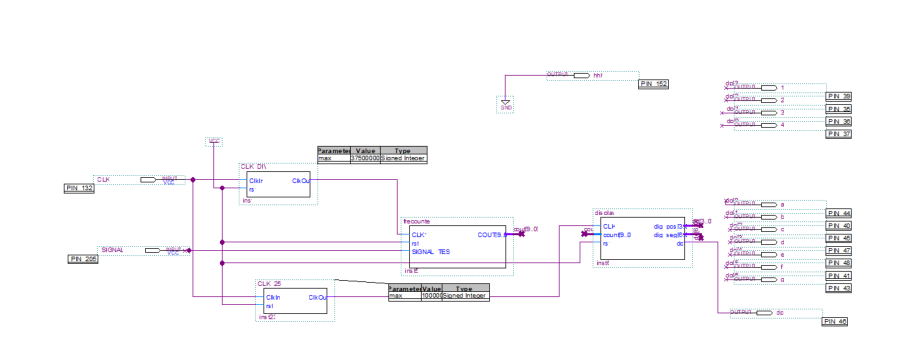
\includegraphics[scale = 0.6 ]{1-1.png}
    \caption{my father}
    \label{img} %方便引用
\end{figure}
%插入方式2
\begin{figure}[H]
    \begin{minipage}[t]{0.45\linewidth}
        \centering
        
\includegraphics[scale = 0.1]{1-1.jpg}
        \caption{father}
    \end{minipage}
        \hfill
    \begin{minipage}[t]{0.5\linewidth}
        \centering
        
\includegraphics[scale = 0.1]{1-1.jpg}
        \caption{s}
    \end{minipage}
\end{figure}


\par{} \textbf{这是一条加粗的句子}

%列表
\begin{itemize}
\item 好玩
\item 好玩
\item 好玩
\item 好玩
\end{itemize}

\begin{enumerate}[(a)]
\item 好玩
\item 好玩
\item 好玩
\item 好玩

\end{enumerate}
%数学表达

$$\left\{
\begin{aligned}
\hat \beta_1 &= \frac{\sum_i(X_i-\overline{X})(Y_i-\overline{Y})}{\sum_i (X_i-\overline{X})^2} \\
\hat \beta_0 &= \overline{Y}-b_1\overline{X} 
\end{aligned}
\right.
$$



$$
\begin{aligned}
    \therefore Var(\hat{ \beta^*}) &=\sum m_i^2Var(Y_i)=\sigma^2\sum m_i^2\\
    &= \sigma^2 \sum(m_i-w_i+w_i)^2\\
    &=\sigma^2\sum(m_i-w_i)^2 +\sigma^2\sum w_i^2+2\sigma^2\sum(m_i-w_i)w_i
\end{aligned}
$$

\begin{displaymath}
    \therefore Var(\hat \beta^*)=\sigma^2\sum(m_i-w_i)^2 +Var(\hat{ \beta_0}) \ge Var(\hat{\beta_0})
\end{displaymath}

%矩阵
\begin{displaymath}
    \Sigma = \begin{pmatrix}
        2.879368  &10.0100 &-1.809053\\
        10.010000 &199.7884& -5.640000\\
        -1.809053 & -5.6400&  3.627658\\
    \end{pmatrix}
\end{displaymath}

%画电路操作
\begin{figure}[H]
    \begin{center}
    \begin{circuitikz}[european resistors]
        \draw (-1, 4) to[open, o-o] (-1, 0);
        \draw (3.5, 4) node[npn](T){}node[]{T};
        \draw(-1, 4)to(T.B);
        \draw ($(T.C)+(3,0)$)coordinate(A) --(T.C);
        \ctikzset{voltage/bump b=22pt,voltage/american label distance=12pt}
        \draw (A) to[open, o-o] (6.5, 0)coordinate(B);
        \draw($(T.C)+(2.2,0)$)to[R=$R_{\rm L}$, *-*](5.7, 0);
        \draw (.5, 0) to [R=$R'_{\rm b1}$, *-](.5, 2)to[vR, -*](.5, 4);
        \node at  (-.1, 3){$R_{\rm W}$};
        \draw (2, 4)to[R=$R_{\rm b2}$, *-*](2, 0);
        \draw (-1, 0)--(B);
        \draw ($(T.C)+(1, 0)$)to[R=$R_{\rm c}$, *-*](4.5, 0);
        \draw(T.E)to[short, -*]($(0,0)!(T.E)!(1,0)$)coordinate(G);
        \node at (G) [rground]{};
        \draw (-1,2)node{$\dot U_I$};
        \draw (7,2.5) node{$\dot U_O$};
    \end{circuitikz}
    \caption{交流等效电路}
    \end{center}
\end{figure}
\par{} 我准备在这里建立一个引用我准备在这里建立一个引用我准备在这里建立一个引用我准备在这里建立一个引用我准备在这里建立一个引用我准备在这里建立一个引用我准备在这里建立一个引用我准备在这里建立一个引用我准备在这里建立一个引用我准备在这里建立一个引用我准备在这里建立一个引用我准备在这里建立一个引用我准备在这里建立一个引用我准备在这里建立一个引用文献\cite{秦玉伟2018一种光电式脉搏信号检测装置}

%链接
\par{}插入一个链接\url{https://cloud.tsinghua.edu.cn/d/f30f6f6678e44818948d/}


%插入各种表格
\begin{table}[H]
    \centering
    \caption{电路刚好起振}
    \begin{tabular}{|l|c|c|c|}
        \hline
         $u_o$&$R_W/k\Omega$&幅值$(V_{pp})/V$&频率/$Hz$\\
        \hline
        理论值 & 10&\diagbox[dir=SW,width=7em,height = 2em]&400 \\
        \hline
        仿真值 &10.65 &1.597& 406.5\\
        \hline
        实测值 &11.83 &0.7&417.4\\
        \hline
      \end{tabular}
\end{table}



\begin{table}[H]
    \begin{tabu}to\textwidth{*{4}{X[c]}}\toprule
        $U_{pp}/V\quad$&示数$\quad$&数模误差\%$\quad$ &模拟误差\%\\ \midrule
        1.00&1.02&2&1.81\\
        1.50&1.51&0.6&0.6\\
        1.80&1.80&0&0.39\\
        1.95&1.96&0.51&0.21\\
        2.00&2.00&0&0.05\\
        2.40&2.39&0.417&0.33\\
        2.50&2.49&0.4&0.36\\
        2.60&2.59&0.38&0.46\\
        2.80&2.78&0.71&0.5\\
        3.00&2.98&0.67&0.73\\
        3.50&3.47&0.86&0.94\\
        3.80&3.76&1.05&1\\
        4.00&3.95&1.25&1.1\\
        4.50&4.44&1.33&1.31\\
        4.80&4.73&1.46&1.46\\
        5.00&4.92&1.6&1.48\\
    \bottomrule
    \end{tabu}
    \caption{1-5V测量数据}
\end{table}


\begin{wrapfigure}{r}{0pt}    
    
\includegraphics[width = 0.4\textwidth]{1-1.jpg}
    \caption{right hand side}
\end{wrapfigure}

我就正常写个段落,他会在左边。我就正常写个段落,他会在左边。我就正常写个段落,他会在左边。我就正常写个段落,他会在左边。我就正常写个段落,他会在左边。我就正常写个段落,他会在左边。我就正常写个段落,他会在左边。我就正常写个段落,他会在左边。我就正常写个段落,他会在左边。我就正常写个段落,他会在左边。我就正常写个段落,他会在左边。我就正常写个段落,他会在左边。我就正常写个段落,他会在左边。我就正常写个段落,他会在左边。我就正常写个段落,他会在左边。我就正常写个段落,他会在左边。我就正常写个段落,他会在左边。我就正常写个段落,他会在左边。我就正常写个段落,他会在左边。我就正常写个段落,他会在左边。

\par{} 我想引用第一张图[\ref{img}]
\bibliographystyle{plain}
\bibliography{latex_template}
\end{document}